\documentclass[tikz,border=3.14pt]{standalone}
\usepackage{../mymacros}
\usepackage{tikz-3dplot}

\definecolor{poliblue1}{RGB}{93,138,168} 
\definecolor{poliblue2}{RGB}{41,76,113}
\definecolor{poliblue3}{RGB}{25,43,67}
\definecolor{orangep}{RGB}{251,146,116}
\definecolor{redp}{RGB}{245,86,91}
\definecolor{greenp}{RGB}{73,165,150}

\begin{document}
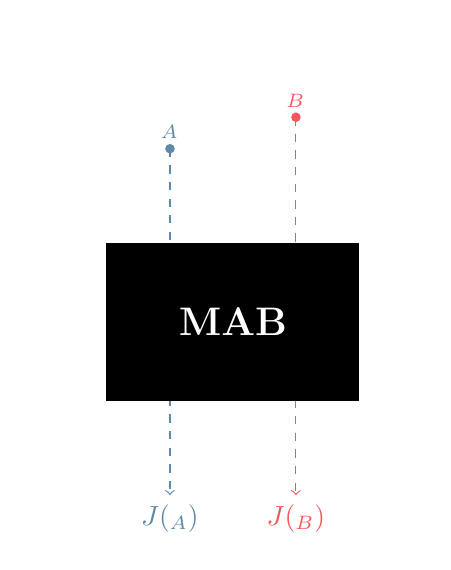
\begin{tikzpicture}[]
\phantom{\draw[] (0,0,0) ellipse (2 and .75) node[right, shift={(1,1)}]{$\Theta$};}
\draw [fill, color=poliblue1] (-0.7,-0.3,0) circle (1.5pt) node[above](a){$\vtheta_A$};
\draw [fill, color=redp] (0.9,0.1,0) circle (1.5pt) node[above](b){$\vtheta_B$};
\phantom{
\draw[] (0,-3.5,0) ellipse (2.5 and .75) node[right, shift={(1,1)}]{$\mathcal{T}$};
\draw[fill, inner color=poliblue1, outer color=white, draw=none, color=white] (-0.7,-3.5,0) ellipse (1.25 and .4) node[above, shift={(1,.2)}, color=poliblue1]{$p_{\vtheta_A}$};
\draw[dashed, color=poliblue1] (a) -- (-0.7,-3.5,0);
\draw[color=poliblue1] (-0.7,-5,0) node (c) {$J(\vtheta_A)$};
\draw[->, dashed, color=poliblue1] (-0.7,-3.5,0) -- (c);
}
\draw[color=poliblue1] (-0.7,-5,0) node (c) {$J(\vtheta_A)$};
\draw[->, dashed, color=poliblue1] (a) -- (c);
\draw[color=redp] (0.9,-5,0) node (d) {$J(\vtheta_B)$};
\draw[->, dashed, color=redp] (b) -- (d);
\draw[fill=black] (-1.5,-1.5,0) rectangle (1.7,-3.5,0) node[pos=.5, color=white]{\bf\Large MAB};
\end{tikzpicture}
\end{document}